% !TEX root=../../thesis.tex

\section{Railway operations} % (fold)
\label{sec:railway_operations}
Major train networks are complex systems with many dynamic effects. The 
Norwegian railroad consists of 4320 km of lines 
\cite[p. 4]{jernbaneverketStatistikk}, transporting 60 million passenger 
journeys and 27 million tons of cargo in 2012
\cite[p. 9]{jernbaneverketStatistikk}. For a rail undertaking, there is a 
constant balance to be struck between capacity, demand, and safe and punctual 
operations. Safety has the highest priority between these concerns, and as 
such this thesis will focus more on capacity and punctual operations.\\

Punctuality is usually divided into two central metrics, punctuality and 
regularity. In the Norwegian railroad, a train is considered punctual or on 
schedule if it operates at planned points in the infrastructure within a 
margin of 3 minutes and 59 seconds, for long distance and cargo trains the 
margin is 5 minutes and 59 seconds. Punctuality (in \%) is the proportion of 
trains that arrives at their final destination within this margin.

Jernbaneverket (see \Vref{sub:subsection_jernbaneverket}) defines regularity (
in \%) as the proportion of trains operated over the number planned in the 
schedule. 

Other derived metrics include uptime, in regards to punctuality, is defined by 
Jernbaneverket from 
the hours of delay\footnote{Hours of delay due to infrastructure excluded 
traffic	management and external conditions} caused by infrastructure relative 
to sum of planned train hours\footnote{Planned train hours (passenger and 
freight trains)} per year.\cite{jernbaneverketPunklighetsTall}
\begin{equation} \label{eq:uptime}
		Uptime =
		\frac
				{
					\text{Train hours - Hours of delay}
				}
				{
					\text{Train hours}
				}\times 100 
\end{equation}\\

In order to continuously improve the quality of the
services, reliability, and punctuality of the railway services, it is important
to monitor train delays their causes  \cite{goverde2011advanced}. 
Train delays can be divided in two types, primary delays where a schedule 
deviation is caused by some disruption at any location due to variations 
within a process; secondary delay is a process time extension caused by 
another train \cite{goverde2005punctuality}.
Analyzing the route conflicts which leads to a primary delays, is necessary in
order to continuously improve the quality of the services, reliability, and 
punctuality of the railway services. An example of a application to analyze the
conflicts is presented by Goverde and Meng \cite{goverde2011advanced}.\\

The operations of the railway system are divided into infrastructure owner and 
rail undertakings that provide transport on the infrastructure. In Norway the 
infrastructure is constructed, operated and maintained by the state owned 
agency Jernbaneverket. The major undertakings operating in Norway  include 
Norges Statsbaner (NSB), NSB Gjøvikbanen, CargoNet, CargoLink, and Flytoget \cite{ wiki:NorwegianRailway}. The undertakings provide exclusively either passenger 
or freight traffic.\\

Due to the size and responsibility of these organizations, there is a need for 
a division of labor and responsibility. This differs between the 
infrastructure owner and the undertakings due to their different business 
areas. Example of their individual organization charts is shown in \Ref{fig:jbv_undertaking_org_map} (undertaking) and \Ref{fig:jbv_infrastructure_org_map} (infrastructure owner).

\begin{figure}[!htbp]
	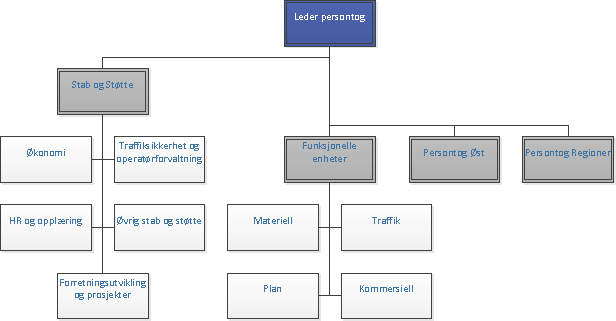
\includegraphics[width=\textwidth,center]{jbv_persontog_orgkart.png}
	\caption[Jernbaneverket undertaking organization]{Jernbaneverket undertaking organization \cite{sintefPresis}}
	\label{fig:jbv_undertaking_org_map}
\end{figure}

\begin{figure}[!htbp]
	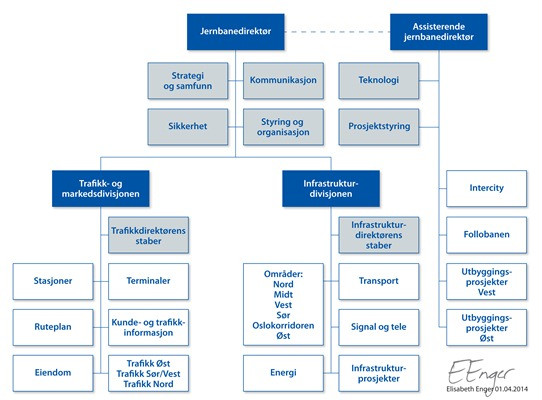
\includegraphics[width=\textwidth,center]{JBV_orgkart.jpg}
	\caption[Jernbaneverket infrastructure organization]{Jernbaneverket infrastructure organization \cite{jernbaneverketOrganisasjon}}
	\label{fig:jbv_infrastructure_org_map}
\end{figure}

To have a safe and punctual operation of the whole system there are
many parts that need to cooperate and interoperate. There is not one unit that
provides safety or punctuality by it self. The cooperation between the 
infrastructure owner and undertakings is also key for a good operation. 

An example of a cooperation both within a company and between several, based on
NSB (\Ref{fig:jbv_undertaking_org_map}) and Jernbaneverket (\Ref{fig:jbv_infrastructure_org_map}), is as follows. The traffic division 
performs the execution of the schedule; the material division maintains and
presents the necessary material to execute the schedule; the planning division
work with planning the long term schedules - which the traffic division
executes; the passenger trains east/region divisions makes personnel 
available, such as train operator, conductor, and line managers. These 
divisions and their cooperation can then be matched against the traffic- and 
marketing division, and infrastructure division in Jernbaneverket, presented in
\Ref{fig:jbv_infrastructure_org_map}.\\

Since most of the railway structure in Norway is single line, most crossings
have to be executed at places where sidetracks have been built, mostly this is
at stations. This means that even though one train may be experiencing delay, 
this delay may be part of a sequence of problems that can be tracked back to a 
seemingly unrelated part of the the network and a perhaps a bad decision there 
\cite{cule2011mining}.
\\

As Landex\cite{landex2009gis} says, there exist few GIS-approaches concerning
visualization of railroad capacity. Both the visualizations shown by Landex and
in \Ref{sect:backgroundExamples} \nameref{sect:backgroundExamples}, 
only seems to take into consideration whether
the trains are delayed, and the amount of delay. \\

% section railway_operations (end)
